
\documentclass[pdf]{beamer}

\mode<presentation>{}

\usetheme{CambridgeUS}

\usepackage[utf8]{inputenc}
\usepackage{tikz}
\usetikzlibrary{positioning}
\usetikzlibrary{calc}

\usepackage{listings}
\lstset{emph={new, val, trait}, emphstyle=\color{red} }
\title{Tower Defense}
\author{Alexis Laouar, R\'emi Oudin, K\'evin Le Run}

\begin{document}

\begin{frame}
  \titlepage
\end{frame}

\begin{frame}
  \frametitle{Plan}
  \tableofcontents
\end{frame}

\section{Fonctionnalit\'es}

\subsection{Tours}
\begin{frame}
  \frametitle{Tours}
  \begin{itemize}
  \item 4 types de tours
  \item Tours qui tirent en zone
  \item Achat et vente de tours
  \end{itemize}
\end{frame}

\begin{frame}[fragile]
    \frametitle{Tours}
    \lstinputlisting{tower.scala}
\end{frame}

\subsection{Ennemis}
\begin{frame}
  \frametitle{Ennemis}
  \begin{itemize}
  \item 5 types d'ennemis
  \item Dont 1 boss et 1 easter egg
  \end{itemize}
\end{frame}

\begin{frame}
    \frametitle{Ennemis}
    \lstinputlisting{bunny.scala}
\end{frame}

\section{Architecture}

\subsection{MVC}

\begin{frame}
  \frametitle{Mod\`ele Vue Contr\^oleur}
  \begin{figure}[h]
    \centering
    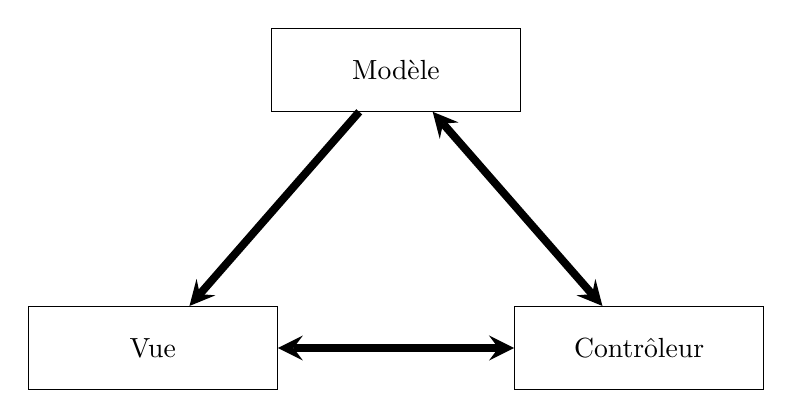
\begin{tikzpicture}[
      elementblock/.style={draw,rectangle,minimum height=3em, minimum width=9em},
      node distance=3cm]
      % Blocks
      \node[elementblock]                                     (view)      {Vue};
      \node[elementblock,right=of view]                       (controller){Contr\^oleur};
      \node[elementblock,above=of {$(view)!0.5!(controller)$}](model)     {Mod\`ele};

      % Arrows
      \draw[         -{stealth},thick,line width=0.1cm] (model) edge (view);
      \draw[{stealth}-{stealth},thick,line width=0.1cm] (model) edge (controller) (controller) edge (view);

    \end{tikzpicture}
    \caption{Modèle-Vue-Contrôleur}
  \end{figure}
\end{frame}

\subsection{Design Patterns}

\begin{frame}
  \frametitle{Type Object}
  Au lieu d'avoir une classe par type d'ennemi : une classe ennemi et une classe
  type d'ennemi
\end{frame}

\section{Le SpawnScheduler}

\subsection{La création de vagues}
\begin{frame}
    \frametitle{Création des vagues}
    \begin{itemize}
        \item Les vagues sont stockées dans un fichier csv
        \item Chaque vague à son fichier, qu'on lit pour stocker dans un buffer
        \item Un programme Caml génère des vagues automatiquement selon des
            facteurs de difficulté.
        \item Un easter egg : Avec une probabilité 1/1000, c'est un lapin doré
            super rapide mais qui rapporte beaucoup d'argent qui apparaît
    \end{itemize}
\end{frame}

\subsection{La gestion d'une vague}
\begin{frame}
    \frametitle{Gestion d'une vague}
        \begin{itemize}
            \item Le SpawnScheduler calcule le temps déroulé depuis le début de
                la vague
            \item Si le temps d'apparition d'un ennemi est inférieur au temps
                déroulé depuis le début de la vague, on le clone depuis le
                SpawnScheduler pour le rajouter dans les ennemis vivants.
        \end{itemize}
    \end{frame}
\section{Conclusion}

\end{document}
